% Created by tikzDevice version 0.12.3 on 2019-09-27 15:50:51
% !TEX encoding = UTF-8 Unicode
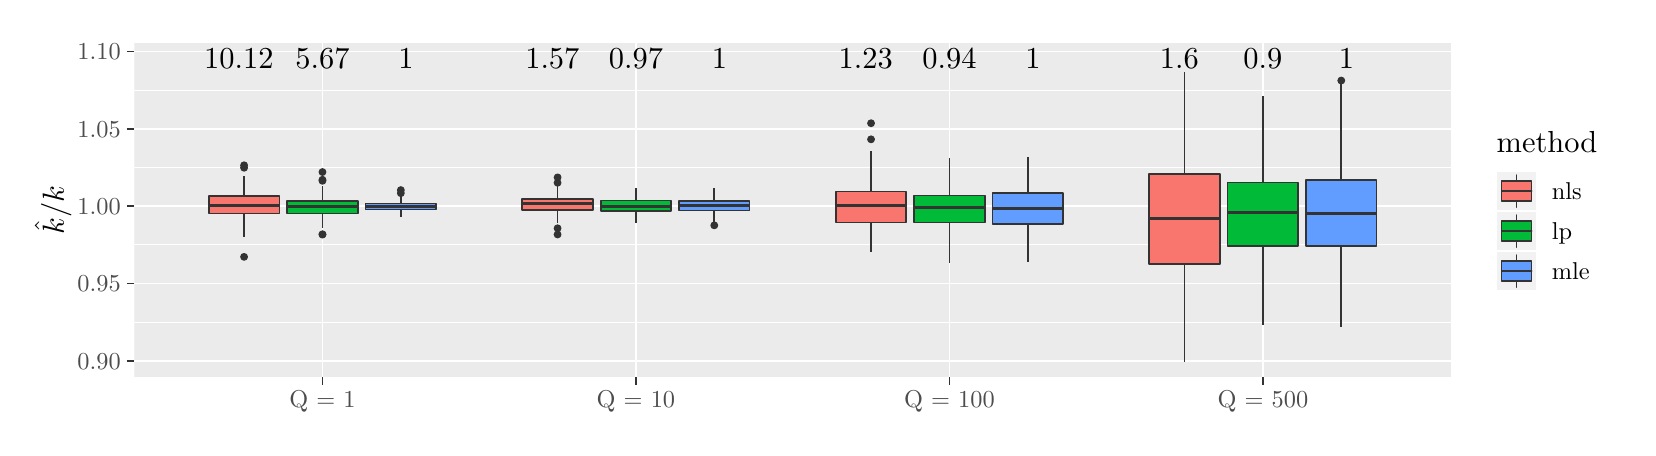
\begin{tikzpicture}[x=1pt,y=1pt]
\definecolor{fillColor}{RGB}{255,255,255}
\path[use as bounding box,fill=fillColor,fill opacity=0.00] (0,0) rectangle (578.16,144.54);
\begin{scope}
\path[clip] (  0.00,  0.00) rectangle (578.16,144.54);
\definecolor{drawColor}{RGB}{255,255,255}
\definecolor{fillColor}{RGB}{255,255,255}

\path[draw=drawColor,line width= 0.6pt,line join=round,line cap=round,fill=fillColor] (  0.00,  0.00) rectangle (578.16,144.54);
\end{scope}
\begin{scope}
\path[clip] ( 38.56, 18.22) rectangle (514.31,139.04);
\definecolor{fillColor}{gray}{0.92}

\path[fill=fillColor] ( 38.56, 18.22) rectangle (514.31,139.04);
\definecolor{drawColor}{RGB}{255,255,255}

\path[draw=drawColor,line width= 0.3pt,line join=round] ( 38.56, 38.08) --
	(514.31, 38.08);

\path[draw=drawColor,line width= 0.3pt,line join=round] ( 38.56, 66.04) --
	(514.31, 66.04);

\path[draw=drawColor,line width= 0.3pt,line join=round] ( 38.56, 94.00) --
	(514.31, 94.00);

\path[draw=drawColor,line width= 0.3pt,line join=round] ( 38.56,121.97) --
	(514.31,121.97);

\path[draw=drawColor,line width= 0.6pt,line join=round] ( 38.56, 24.10) --
	(514.31, 24.10);

\path[draw=drawColor,line width= 0.6pt,line join=round] ( 38.56, 52.06) --
	(514.31, 52.06);

\path[draw=drawColor,line width= 0.6pt,line join=round] ( 38.56, 80.02) --
	(514.31, 80.02);

\path[draw=drawColor,line width= 0.6pt,line join=round] ( 38.56,107.99) --
	(514.31,107.99);

\path[draw=drawColor,line width= 0.6pt,line join=round] ( 38.56,135.95) --
	(514.31,135.95);

\path[draw=drawColor,line width= 0.6pt,line join=round] (106.52, 18.22) --
	(106.52,139.04);

\path[draw=drawColor,line width= 0.6pt,line join=round] (219.79, 18.22) --
	(219.79,139.04);

\path[draw=drawColor,line width= 0.6pt,line join=round] (333.07, 18.22) --
	(333.07,139.04);

\path[draw=drawColor,line width= 0.6pt,line join=round] (446.34, 18.22) --
	(446.34,139.04);
\definecolor{drawColor}{gray}{0.20}
\definecolor{fillColor}{gray}{0.20}

\path[draw=drawColor,line width= 0.4pt,line join=round,line cap=round,fill=fillColor] ( 78.20, 61.72) circle (  1.21);

\path[draw=drawColor,line width= 0.4pt,line join=round,line cap=round,fill=fillColor] ( 78.20, 93.92) circle (  1.21);

\path[draw=drawColor,line width= 0.4pt,line join=round,line cap=round,fill=fillColor] ( 78.20, 94.81) circle (  1.21);

\path[draw=drawColor,line width= 0.6pt,line join=round] ( 78.20, 83.65) -- ( 78.20, 90.92);

\path[draw=drawColor,line width= 0.6pt,line join=round] ( 78.20, 77.42) -- ( 78.20, 68.94);
\definecolor{fillColor}{RGB}{248,118,109}

\path[draw=drawColor,line width= 0.6pt,line join=round,line cap=round,fill=fillColor] ( 65.46, 83.65) --
	( 65.46, 77.42) --
	( 90.94, 77.42) --
	( 90.94, 83.65) --
	( 65.46, 83.65) --
	cycle;

\path[draw=drawColor,line width= 1.1pt,line join=round] ( 65.46, 80.24) -- ( 90.94, 80.24);
\definecolor{fillColor}{gray}{0.20}

\path[draw=drawColor,line width= 0.4pt,line join=round,line cap=round,fill=fillColor] (106.52, 89.58) circle (  1.21);

\path[draw=drawColor,line width= 0.4pt,line join=round,line cap=round,fill=fillColor] (106.52, 89.20) circle (  1.21);

\path[draw=drawColor,line width= 0.4pt,line join=round,line cap=round,fill=fillColor] (106.52, 69.87) circle (  1.21);

\path[draw=drawColor,line width= 0.4pt,line join=round,line cap=round,fill=fillColor] (106.52, 69.78) circle (  1.21);

\path[draw=drawColor,line width= 0.4pt,line join=round,line cap=round,fill=fillColor] (106.52, 92.37) circle (  1.21);

\path[draw=drawColor,line width= 0.6pt,line join=round] (106.52, 81.92) -- (106.52, 87.39);

\path[draw=drawColor,line width= 0.6pt,line join=round] (106.52, 77.40) -- (106.52, 71.98);
\definecolor{fillColor}{RGB}{0,186,56}

\path[draw=drawColor,line width= 0.6pt,line join=round,line cap=round,fill=fillColor] ( 93.78, 81.92) --
	( 93.78, 77.40) --
	(119.26, 77.40) --
	(119.26, 81.92) --
	( 93.78, 81.92) --
	cycle;

\path[draw=drawColor,line width= 1.1pt,line join=round] ( 93.78, 79.80) -- (119.26, 79.80);
\definecolor{fillColor}{gray}{0.20}

\path[draw=drawColor,line width= 0.4pt,line join=round,line cap=round,fill=fillColor] (134.84, 84.74) circle (  1.21);

\path[draw=drawColor,line width= 0.4pt,line join=round,line cap=round,fill=fillColor] (134.84, 85.85) circle (  1.21);

\path[draw=drawColor,line width= 0.6pt,line join=round] (134.84, 80.96) -- (134.84, 83.87);

\path[draw=drawColor,line width= 0.6pt,line join=round] (134.84, 78.86) -- (134.84, 76.19);
\definecolor{fillColor}{RGB}{97,156,255}

\path[draw=drawColor,line width= 0.6pt,line join=round,line cap=round,fill=fillColor] (122.09, 80.96) --
	(122.09, 78.86) --
	(147.58, 78.86) --
	(147.58, 80.96) --
	(122.09, 80.96) --
	cycle;

\path[draw=drawColor,line width= 1.1pt,line join=round] (122.09, 79.96) -- (147.58, 79.96);
\definecolor{fillColor}{gray}{0.20}

\path[draw=drawColor,line width= 0.4pt,line join=round,line cap=round,fill=fillColor] (191.48, 72.05) circle (  1.21);

\path[draw=drawColor,line width= 0.4pt,line join=round,line cap=round,fill=fillColor] (191.48, 88.50) circle (  1.21);

\path[draw=drawColor,line width= 0.4pt,line join=round,line cap=round,fill=fillColor] (191.48, 90.44) circle (  1.21);

\path[draw=drawColor,line width= 0.4pt,line join=round,line cap=round,fill=fillColor] (191.48, 69.81) circle (  1.21);

\path[draw=drawColor,line width= 0.6pt,line join=round] (191.48, 82.59) -- (191.48, 87.56);

\path[draw=drawColor,line width= 0.6pt,line join=round] (191.48, 78.76) -- (191.48, 73.82);
\definecolor{fillColor}{RGB}{248,118,109}

\path[draw=drawColor,line width= 0.6pt,line join=round,line cap=round,fill=fillColor] (178.73, 82.59) --
	(178.73, 78.76) --
	(204.22, 78.76) --
	(204.22, 82.59) --
	(178.73, 82.59) --
	cycle;

\path[draw=drawColor,line width= 1.1pt,line join=round] (178.73, 80.94) -- (204.22, 80.94);

\path[draw=drawColor,line width= 0.6pt,line join=round] (219.79, 82.13) -- (219.79, 86.67);

\path[draw=drawColor,line width= 0.6pt,line join=round] (219.79, 78.39) -- (219.79, 74.06);
\definecolor{fillColor}{RGB}{0,186,56}

\path[draw=drawColor,line width= 0.6pt,line join=round,line cap=round,fill=fillColor] (207.05, 82.13) --
	(207.05, 78.39) --
	(232.54, 78.39) --
	(232.54, 82.13) --
	(207.05, 82.13) --
	cycle;

\path[draw=drawColor,line width= 1.1pt,line join=round] (207.05, 80.05) -- (232.54, 80.05);
\definecolor{fillColor}{gray}{0.20}

\path[draw=drawColor,line width= 0.4pt,line join=round,line cap=round,fill=fillColor] (248.11, 73.11) circle (  1.21);

\path[draw=drawColor,line width= 0.6pt,line join=round] (248.11, 81.91) -- (248.11, 86.73);

\path[draw=drawColor,line width= 0.6pt,line join=round] (248.11, 78.46) -- (248.11, 73.69);
\definecolor{fillColor}{RGB}{97,156,255}

\path[draw=drawColor,line width= 0.6pt,line join=round,line cap=round,fill=fillColor] (235.37, 81.91) --
	(235.37, 78.46) --
	(260.86, 78.46) --
	(260.86, 81.91) --
	(235.37, 81.91) --
	cycle;

\path[draw=drawColor,line width= 1.1pt,line join=round] (235.37, 80.21) -- (260.86, 80.21);
\definecolor{fillColor}{gray}{0.20}

\path[draw=drawColor,line width= 0.4pt,line join=round,line cap=round,fill=fillColor] (304.75,104.19) circle (  1.21);

\path[draw=drawColor,line width= 0.4pt,line join=round,line cap=round,fill=fillColor] (304.75,110.01) circle (  1.21);

\path[draw=drawColor,line width= 0.6pt,line join=round] (304.75, 85.36) -- (304.75, 99.94);

\path[draw=drawColor,line width= 0.6pt,line join=round] (304.75, 74.19) -- (304.75, 63.55);
\definecolor{fillColor}{RGB}{248,118,109}

\path[draw=drawColor,line width= 0.6pt,line join=round,line cap=round,fill=fillColor] (292.01, 85.36) --
	(292.01, 74.19) --
	(317.49, 74.19) --
	(317.49, 85.36) --
	(292.01, 85.36) --
	cycle;

\path[draw=drawColor,line width= 1.1pt,line join=round] (292.01, 80.42) -- (317.49, 80.42);

\path[draw=drawColor,line width= 0.6pt,line join=round] (333.07, 83.93) -- (333.07, 97.28);

\path[draw=drawColor,line width= 0.6pt,line join=round] (333.07, 74.16) -- (333.07, 59.51);
\definecolor{fillColor}{RGB}{0,186,56}

\path[draw=drawColor,line width= 0.6pt,line join=round,line cap=round,fill=fillColor] (320.33, 83.93) --
	(320.33, 74.16) --
	(345.81, 74.16) --
	(345.81, 83.93) --
	(320.33, 83.93) --
	cycle;

\path[draw=drawColor,line width= 1.1pt,line join=round] (320.33, 79.44) -- (345.81, 79.44);

\path[draw=drawColor,line width= 0.6pt,line join=round] (361.39, 84.82) -- (361.39, 97.97);

\path[draw=drawColor,line width= 0.6pt,line join=round] (361.39, 73.68) -- (361.39, 59.84);
\definecolor{fillColor}{RGB}{97,156,255}

\path[draw=drawColor,line width= 0.6pt,line join=round,line cap=round,fill=fillColor] (348.64, 84.82) --
	(348.64, 73.68) --
	(374.13, 73.68) --
	(374.13, 84.82) --
	(348.64, 84.82) --
	cycle;

\path[draw=drawColor,line width= 1.1pt,line join=round] (348.64, 79.23) -- (374.13, 79.23);

\path[draw=drawColor,line width= 0.6pt,line join=round] (418.02, 91.68) -- (418.02,128.68);

\path[draw=drawColor,line width= 0.6pt,line join=round] (418.02, 59.14) -- (418.02, 23.71);
\definecolor{fillColor}{RGB}{248,118,109}

\path[draw=drawColor,line width= 0.6pt,line join=round,line cap=round,fill=fillColor] (405.28, 91.68) --
	(405.28, 59.14) --
	(430.77, 59.14) --
	(430.77, 91.68) --
	(405.28, 91.68) --
	cycle;

\path[draw=drawColor,line width= 1.1pt,line join=round] (405.28, 75.56) -- (430.77, 75.56);

\path[draw=drawColor,line width= 0.6pt,line join=round] (446.34, 88.56) -- (446.34,119.88);

\path[draw=drawColor,line width= 0.6pt,line join=round] (446.34, 65.64) -- (446.34, 37.01);
\definecolor{fillColor}{RGB}{0,186,56}

\path[draw=drawColor,line width= 0.6pt,line join=round,line cap=round,fill=fillColor] (433.60, 88.56) --
	(433.60, 65.64) --
	(459.09, 65.64) --
	(459.09, 88.56) --
	(433.60, 88.56) --
	cycle;

\path[draw=drawColor,line width= 1.1pt,line join=round] (433.60, 77.88) -- (459.09, 77.88);
\definecolor{fillColor}{gray}{0.20}

\path[draw=drawColor,line width= 0.4pt,line join=round,line cap=round,fill=fillColor] (474.66,125.43) circle (  1.21);

\path[draw=drawColor,line width= 0.6pt,line join=round] (474.66, 89.52) -- (474.66,124.25);

\path[draw=drawColor,line width= 0.6pt,line join=round] (474.66, 65.76) -- (474.66, 36.38);
\definecolor{fillColor}{RGB}{97,156,255}

\path[draw=drawColor,line width= 0.6pt,line join=round,line cap=round,fill=fillColor] (461.92, 89.52) --
	(461.92, 65.76) --
	(487.40, 65.76) --
	(487.40, 89.52) --
	(461.92, 89.52) --
	cycle;

\path[draw=drawColor,line width= 1.1pt,line join=round] (461.92, 77.56) -- (487.40, 77.56);
\definecolor{drawColor}{RGB}{0,0,0}

\node[text=drawColor,anchor=base,inner sep=0pt, outer sep=0pt, scale=  1.10] at (136.73,129.75) {1};

\node[text=drawColor,anchor=base,inner sep=0pt, outer sep=0pt, scale=  1.10] at (106.52,129.75) {5.67};

\node[text=drawColor,anchor=base,inner sep=0pt, outer sep=0pt, scale=  1.10] at ( 76.31,129.75) {10.12};

\node[text=drawColor,anchor=base,inner sep=0pt, outer sep=0pt, scale=  1.10] at (250.00,129.75) {1};

\node[text=drawColor,anchor=base,inner sep=0pt, outer sep=0pt, scale=  1.10] at (219.79,129.75) {0.97};

\node[text=drawColor,anchor=base,inner sep=0pt, outer sep=0pt, scale=  1.10] at (189.59,129.75) {1.57};

\node[text=drawColor,anchor=base,inner sep=0pt, outer sep=0pt, scale=  1.10] at (363.28,129.75) {1};

\node[text=drawColor,anchor=base,inner sep=0pt, outer sep=0pt, scale=  1.10] at (333.07,129.75) {0.94};

\node[text=drawColor,anchor=base,inner sep=0pt, outer sep=0pt, scale=  1.10] at (302.86,129.75) {1.23};

\node[text=drawColor,anchor=base,inner sep=0pt, outer sep=0pt, scale=  1.10] at (476.55,129.75) {1};

\node[text=drawColor,anchor=base,inner sep=0pt, outer sep=0pt, scale=  1.10] at (446.34,129.75) {0.9};

\node[text=drawColor,anchor=base,inner sep=0pt, outer sep=0pt, scale=  1.10] at (416.14,129.75) {1.6};
\end{scope}
\begin{scope}
\path[clip] (  0.00,  0.00) rectangle (578.16,144.54);
\definecolor{drawColor}{gray}{0.30}

\node[text=drawColor,anchor=base east,inner sep=0pt, outer sep=0pt, scale=  0.88] at ( 33.61, 21.07) {0.90};

\node[text=drawColor,anchor=base east,inner sep=0pt, outer sep=0pt, scale=  0.88] at ( 33.61, 49.03) {0.95};

\node[text=drawColor,anchor=base east,inner sep=0pt, outer sep=0pt, scale=  0.88] at ( 33.61, 76.99) {1.00};

\node[text=drawColor,anchor=base east,inner sep=0pt, outer sep=0pt, scale=  0.88] at ( 33.61,104.96) {1.05};

\node[text=drawColor,anchor=base east,inner sep=0pt, outer sep=0pt, scale=  0.88] at ( 33.61,132.92) {1.10};
\end{scope}
\begin{scope}
\path[clip] (  0.00,  0.00) rectangle (578.16,144.54);
\definecolor{drawColor}{gray}{0.20}

\path[draw=drawColor,line width= 0.6pt,line join=round] ( 35.81, 24.10) --
	( 38.56, 24.10);

\path[draw=drawColor,line width= 0.6pt,line join=round] ( 35.81, 52.06) --
	( 38.56, 52.06);

\path[draw=drawColor,line width= 0.6pt,line join=round] ( 35.81, 80.02) --
	( 38.56, 80.02);

\path[draw=drawColor,line width= 0.6pt,line join=round] ( 35.81,107.99) --
	( 38.56,107.99);

\path[draw=drawColor,line width= 0.6pt,line join=round] ( 35.81,135.95) --
	( 38.56,135.95);
\end{scope}
\begin{scope}
\path[clip] (  0.00,  0.00) rectangle (578.16,144.54);
\definecolor{drawColor}{gray}{0.20}

\path[draw=drawColor,line width= 0.6pt,line join=round] (106.52, 15.47) --
	(106.52, 18.22);

\path[draw=drawColor,line width= 0.6pt,line join=round] (219.79, 15.47) --
	(219.79, 18.22);

\path[draw=drawColor,line width= 0.6pt,line join=round] (333.07, 15.47) --
	(333.07, 18.22);

\path[draw=drawColor,line width= 0.6pt,line join=round] (446.34, 15.47) --
	(446.34, 18.22);
\end{scope}
\begin{scope}
\path[clip] (  0.00,  0.00) rectangle (578.16,144.54);
\definecolor{drawColor}{gray}{0.30}

\node[text=drawColor,anchor=base,inner sep=0pt, outer sep=0pt, scale=  0.88] at (106.52,  7.21) {Q = 1};

\node[text=drawColor,anchor=base,inner sep=0pt, outer sep=0pt, scale=  0.88] at (219.79,  7.21) {Q = 10};

\node[text=drawColor,anchor=base,inner sep=0pt, outer sep=0pt, scale=  0.88] at (333.07,  7.21) {Q = 100};

\node[text=drawColor,anchor=base,inner sep=0pt, outer sep=0pt, scale=  0.88] at (446.34,  7.21) {Q = 500};
\end{scope}
\begin{scope}
\path[clip] (  0.00,  0.00) rectangle (578.16,144.54);
\definecolor{drawColor}{RGB}{0,0,0}

\node[text=drawColor,rotate= 90.00,anchor=base,inner sep=0pt, outer sep=0pt, scale=  1.10] at ( 13.08, 78.63) {$\hat{k}/k$};
\end{scope}
\begin{scope}
\path[clip] (  0.00,  0.00) rectangle (578.16,144.54);
\definecolor{fillColor}{RGB}{255,255,255}

\path[fill=fillColor] (525.31, 43.84) rectangle (572.66,113.42);
\end{scope}
\begin{scope}
\path[clip] (  0.00,  0.00) rectangle (578.16,144.54);
\definecolor{drawColor}{RGB}{0,0,0}

\node[text=drawColor,anchor=base west,inner sep=0pt, outer sep=0pt, scale=  1.10] at (530.81, 99.27) {method};
\end{scope}
\begin{scope}
\path[clip] (  0.00,  0.00) rectangle (578.16,144.54);
\definecolor{drawColor}{RGB}{255,255,255}
\definecolor{fillColor}{gray}{0.95}

\path[draw=drawColor,line width= 0.6pt,line join=round,line cap=round,fill=fillColor] (530.81, 78.25) rectangle (545.26, 92.70);
\end{scope}
\begin{scope}
\path[clip] (  0.00,  0.00) rectangle (578.16,144.54);
\definecolor{drawColor}{gray}{0.20}

\path[draw=drawColor,line width= 0.6pt,line join=round,line cap=round] (538.03, 79.70) --
	(538.03, 81.86);

\path[draw=drawColor,line width= 0.6pt,line join=round,line cap=round] (538.03, 89.09) --
	(538.03, 91.26);
\definecolor{fillColor}{RGB}{248,118,109}

\path[draw=drawColor,line width= 0.6pt,line join=round,line cap=round,fill=fillColor] (532.61, 81.86) rectangle (543.45, 89.09);

\path[draw=drawColor,line width= 0.6pt,line join=round,line cap=round] (532.61, 85.48) --
	(543.45, 85.48);
\end{scope}
\begin{scope}
\path[clip] (  0.00,  0.00) rectangle (578.16,144.54);
\definecolor{drawColor}{RGB}{255,255,255}
\definecolor{fillColor}{gray}{0.95}

\path[draw=drawColor,line width= 0.6pt,line join=round,line cap=round,fill=fillColor] (530.81, 63.80) rectangle (545.26, 78.25);
\end{scope}
\begin{scope}
\path[clip] (  0.00,  0.00) rectangle (578.16,144.54);
\definecolor{drawColor}{gray}{0.20}

\path[draw=drawColor,line width= 0.6pt,line join=round,line cap=round] (538.03, 65.24) --
	(538.03, 67.41);

\path[draw=drawColor,line width= 0.6pt,line join=round,line cap=round] (538.03, 74.64) --
	(538.03, 76.81);
\definecolor{fillColor}{RGB}{0,186,56}

\path[draw=drawColor,line width= 0.6pt,line join=round,line cap=round,fill=fillColor] (532.61, 67.41) rectangle (543.45, 74.64);

\path[draw=drawColor,line width= 0.6pt,line join=round,line cap=round] (532.61, 71.02) --
	(543.45, 71.02);
\end{scope}
\begin{scope}
\path[clip] (  0.00,  0.00) rectangle (578.16,144.54);
\definecolor{drawColor}{RGB}{255,255,255}
\definecolor{fillColor}{gray}{0.95}

\path[draw=drawColor,line width= 0.6pt,line join=round,line cap=round,fill=fillColor] (530.81, 49.34) rectangle (545.26, 63.80);
\end{scope}
\begin{scope}
\path[clip] (  0.00,  0.00) rectangle (578.16,144.54);
\definecolor{drawColor}{gray}{0.20}

\path[draw=drawColor,line width= 0.6pt,line join=round,line cap=round] (538.03, 50.79) --
	(538.03, 52.96);

\path[draw=drawColor,line width= 0.6pt,line join=round,line cap=round] (538.03, 60.18) --
	(538.03, 62.35);
\definecolor{fillColor}{RGB}{97,156,255}

\path[draw=drawColor,line width= 0.6pt,line join=round,line cap=round,fill=fillColor] (532.61, 52.96) rectangle (543.45, 60.18);

\path[draw=drawColor,line width= 0.6pt,line join=round,line cap=round] (532.61, 56.57) --
	(543.45, 56.57);
\end{scope}
\begin{scope}
\path[clip] (  0.00,  0.00) rectangle (578.16,144.54);
\definecolor{drawColor}{RGB}{0,0,0}

\node[text=drawColor,anchor=base west,inner sep=0pt, outer sep=0pt, scale=  0.88] at (550.76, 82.45) {nls};
\end{scope}
\begin{scope}
\path[clip] (  0.00,  0.00) rectangle (578.16,144.54);
\definecolor{drawColor}{RGB}{0,0,0}

\node[text=drawColor,anchor=base west,inner sep=0pt, outer sep=0pt, scale=  0.88] at (550.76, 67.99) {lp};
\end{scope}
\begin{scope}
\path[clip] (  0.00,  0.00) rectangle (578.16,144.54);
\definecolor{drawColor}{RGB}{0,0,0}

\node[text=drawColor,anchor=base west,inner sep=0pt, outer sep=0pt, scale=  0.88] at (550.76, 53.54) {mle};
\end{scope}
\end{tikzpicture}
